\documentclass[a4paper]{article}
\oddsidemargin -0.2cm
\evensidemargin -1.2cm
\textwidth 17cm
\headheight 2.2cm
\topmargin -4cm
\textheight 25cm
\footskip 15pt
\usepackage[utf8]{inputenc}
\usepackage{amsmath}
\usepackage{amssymb}
\usepackage{multicol}
\usepackage{hyperref}
\usepackage{enumitem}
\usepackage{blindtext}
\usepackage{graphicx}
\graphicspath{ {figures/} }

\begin{document}

\author{Anthony Liu}
\title{Predicting solar installation rates in different locations using demographic data}
\maketitle

\tableofcontents

\section{Introduction}

The central problem that the analysis in this report will attempt to address is "Can we predict solar installation rates in the different local government areas of Australia using demographic data?". As the effects of global climate change are becoming better understood, the move towards renewable energy sources has become an important focus \cite{ipcc}. Solar energy is emerging as one of the most popular forms of renewable energy for reasons such as decreasing costs, environmental ethics, health, government incentives and accessibility \cite{pew, seia}. \\

Australia is in a particularly privileged position to have some of the best solar energy resources in the world \cite{geogov}. Being able to answer the proposed question may lead to insights which guide policy, investment or further research to better utilise this natural resource. Given that installation of solar constitutes a purchase and purchases are made by individuals under their own unique circumstances, there is good reason to believe that demographic factors (such as financial status, dwelling structure, education, etc.) may affect installation rates. In this analysis we limit our scope to prediction of solar installation rates in each local government area (LGA) based on available demographic data. Questions of inference such as which specific demographic factors are related to installation rates are not considered. \\

Parties who may be interested in this problem include policy makers, investors and researchers. Reliable predictions on installation rates may guide projections and highlight both the level and content of policy intervention justified in affecting solar uptake. Also, investors in the solar industry hold an advantage if they have reliable guidance on which local government areas in the future (accounting for demographic shifts) are likely to install solar. Finally, results from attempting to answer this question may lead to new lines of inquiry among researchers (e.g. if we can indeed predict installation rates then that provides justification to then do further research on which exact demographic factors have an effect).

\section{Data}

To answer our problem we use two separate types of data: data regarding solar installation rates in each LGA and data regarding demographics in each LGA. We obtained our first dataset on solar installations from the Australian Photovoltaic Institute \cite{pvdata}. The Australian Photovoltatic Institute (APVI) is a not-for-profit company whose stated objective is to "Support the increased development and use of PV via research, analysis and information" \cite{apvi}. The photovoltaic (PV) data by the APVI was compiled from Australian government body sources: PV installation data came from the Clean Energy Regulator \cite{pvdata, ceg} and attached LGA data was from the Australian Bureau of Statistics (ABS) \cite{pvdata, abspv}. Of particular interest to this analysis is the density variable, an estimate of the percentage of dwellings in each LGA which have installed solar systems. \\

Detailed demographic data on each LGA including socio-economic indicators, dwelling structure, age, sex, cultural background, education and employment was also obtained from the ABS \cite{abs}. Figures \ref{fig:fig1} and \ref{fig:fig2} provide a preview of how the socio-economic indicators and education/employment data look on the ABS website respectively. These entries are later wrangled into an appropriate format and act as individual features/predictors of a machine learning algorithm to predict density (i.e. solar installation rate in each LGA). We restricted our use of demographic information to only that recorded by the ABS in the year 2016 as this year contained the most complete data (the last census took place in 2016).

\begin{figure}
\centering
  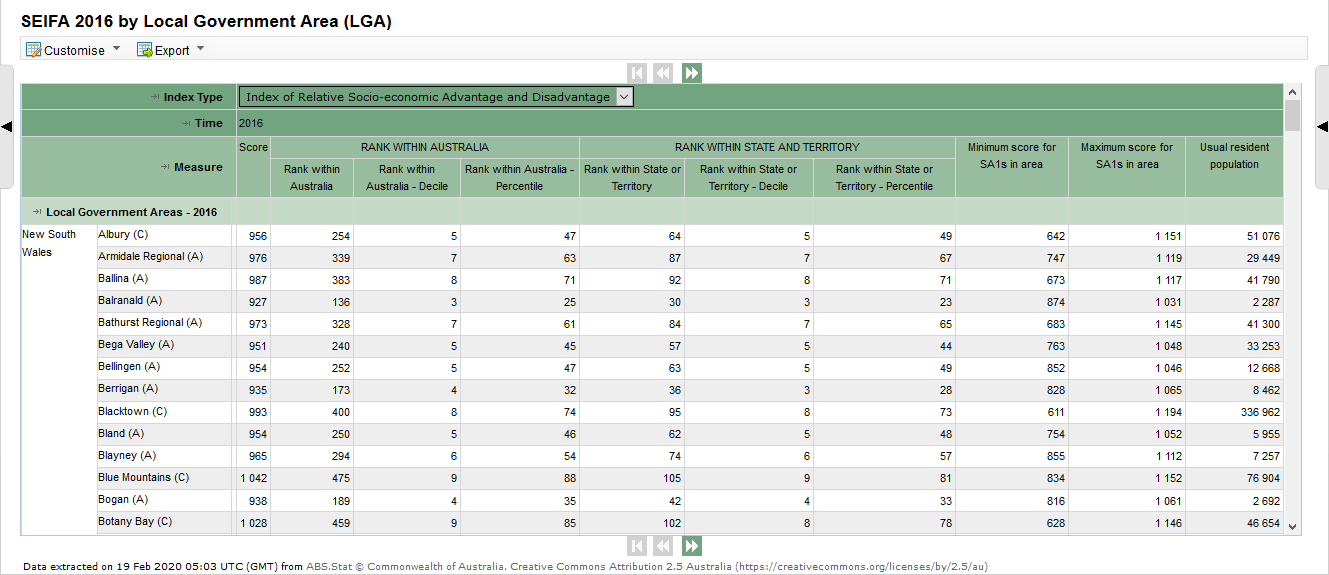
\includegraphics[width=\linewidth]{fig1.png}
  \caption{A preview of the socio-economic indicators dataset on the ABS website, prior to exporting as a CSV file and performing data wrangling.}
  \label{fig:fig1}
\end{figure}

\begin{figure}
\centering
  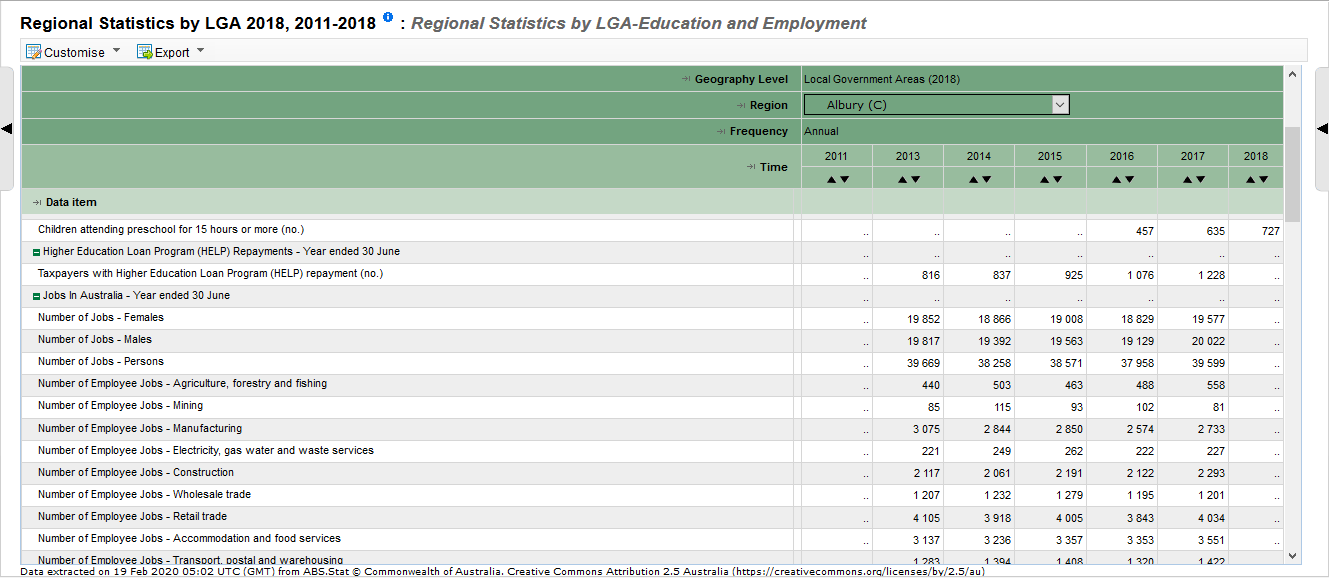
\includegraphics[width=\linewidth]{fig2.png}
  \caption{A preview of the education and employment dataset on the ABS website, prior to exporting as a CSV file and performing data wrangling.}
  \label{fig:fig2}
\end{figure}

\section{Methodology}

\subsection{Data wrangling}

The data obtained from the APVI and ABS were loaded in their raw form using Python 3.7.4. The APVI data contained information including number of installations, total energy capacity, and breakdowns of installations by energy capacity (see Figure \ref{fig:fig3}). As our problem was to predict solar installation rates in each LGA, only information pertaining to the density of installations was used in this analysis (see Figure \ref{fig:fig4}). \\

\begin{figure}
\centering
  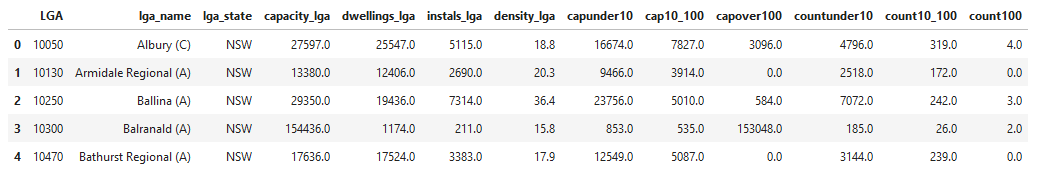
\includegraphics[width=\linewidth]{fig3.png}
  \caption{Solar installation data by the APVI in its raw form upon being loaded.}
  \label{fig:fig3}
\end{figure}

\begin{figure}
\centering
  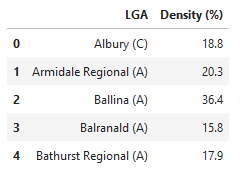
\includegraphics{fig4.png}
  \caption{Solar installation data by the APVI after cleaning. Only the LGA and Density (percentage of dwellings with installed solar) variables were retained.}
  \label{fig:fig4}
\end{figure}

The demographic data from the ABS in its raw form also contained excessive information but we defer the removal of excess information to our principal components analysis later on. We choose to temporarily include all demographic indicators and simply perform a transformation on the data so that it is in a format appropriate for merging with our solar installation data. Figures 5 and 6 demonstrate the transformation performed on the education and employment dataset from the ABS. \\

\begin{figure}
\centering
  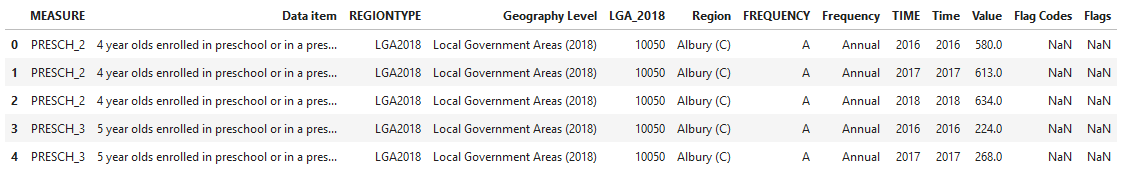
\includegraphics[width=\linewidth]{fig5.png}
  \caption{The educational demographic data from the ABS in its raw form.}
  \label{fig:fig5}
\end{figure}

\begin{figure}
\centering
  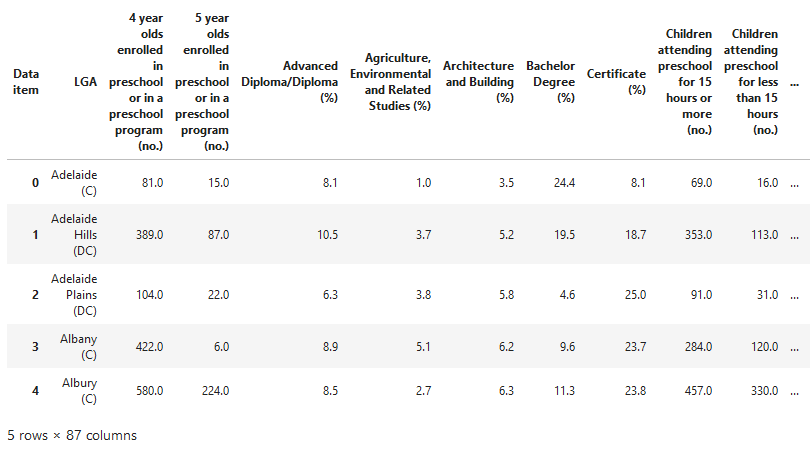
\includegraphics[width=\linewidth]{fig6.png}
  \caption{The education and employment demographic data from the ABS after transformation. There are 87 columns in total, corresponding to 86 predictors (LGA is not used as a predictor). Similar transformations are performed on the other demographic datasets from the ABS.}
  \label{fig:fig6}
\end{figure}

Similar transformations were performed on the SEIFA socio-economic indices, population  and dwelling structure datasets from the ABS. These demographic datasets were then combined with the solar installation dataset to form a combined dataframe where the LGA was the index, the density (our response) was the first column, and all the predictors made up the remaining columns (see Figure \ref{fig:fig7}). The dataframe is now in a "tidy" format where each row is an observation and each column is a variable, a standard which allows for easier data manipulation and analysis \cite{tidy}.

\begin{figure}
\centering
  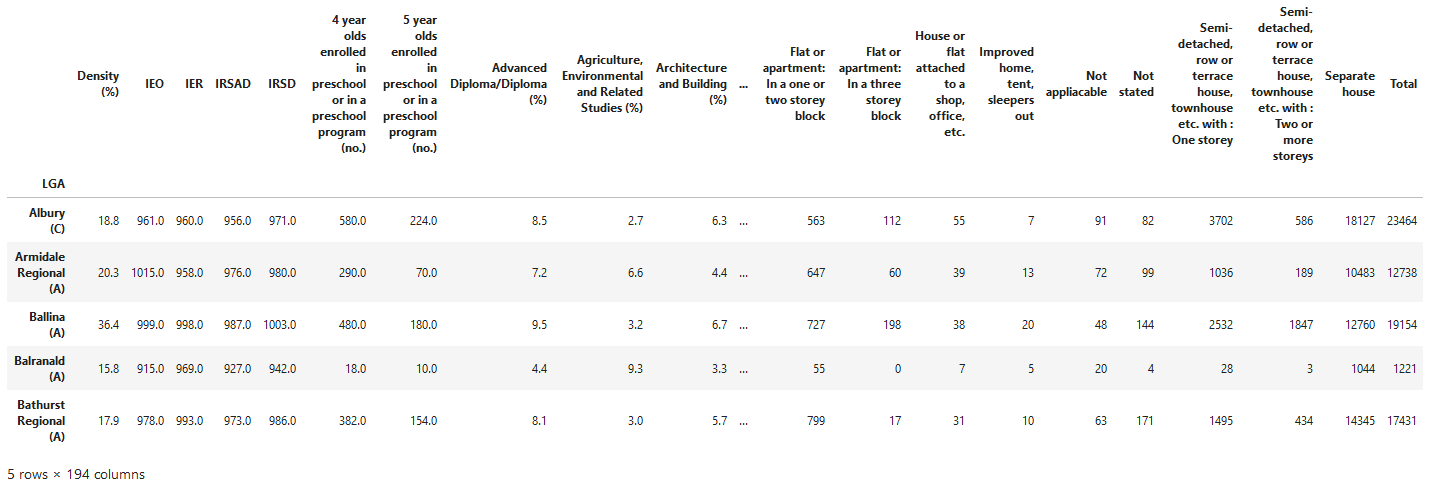
\includegraphics[width=\linewidth]{fig7.png}
  \caption{The combined dataframe containing Density, the response we are trying to predict in this analysis, in the first column, and demographic predictors in the remaining columns.}
  \label{fig:fig7}
\end{figure}

\subsection{Exploratory data analysis}

Within our exploratory data analysis, we computed summary statistics of the combined dataframe to look for any anomalies (see Figure \ref{fig:fig8}). We also explored the effect on dataset size when dropping missing values. The dataset size at this point was 481 rows by 194 columns, so the number of observations (rows) we had were quite small considering the number of predictors we had. We found that dropping rows or columns with missing values resulted in too big of a decrease in dataset size. We also looked at the number of missing values each column had and found a majority only had a few missing values. There did exist other columns, however, which had so many missing values that imputing values into these would have significantly changed predictor data. We elected here to impute the median values for those 125 columns which had less than only 3 missing values, and drop the remaining columns. 

\begin{figure}
\centering
  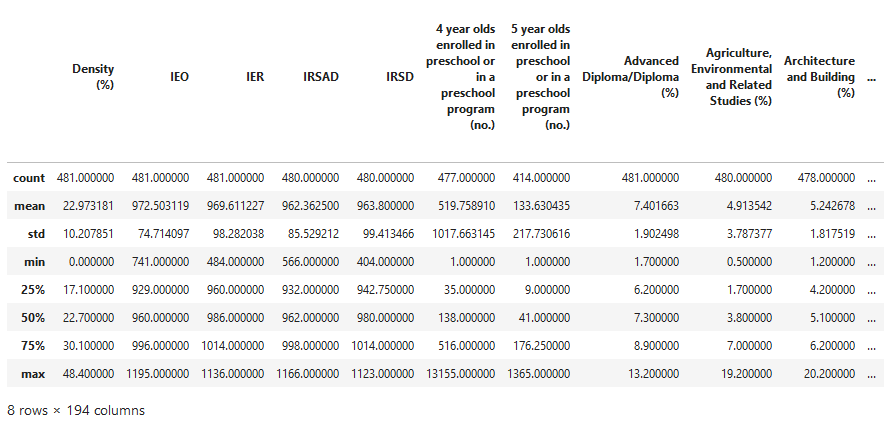
\includegraphics[width=\linewidth]{fig8.png}
  \caption{Summary statistics of the combined dataframe (prior to imputing and removing missing values).}
  \label{fig:fig8}
\end{figure}

\subsection{Preprocessing: train-test split and principal components analysis}

A train-test split of 70-30 was performed on the combined dataframe. We temporarily set aside our test set without referring to it in order to avoid introducing bias later when using the test set for model evaluation. Given that our dataset at this point still had a significant number of predictors relative to observations, we performed a dimension reduction in such a way so as to reduce the number of predictors while retaining most of their information. There is good reason to suspect that there are many redundant predictors in this dataframe given the large number of predictors and that predictors like the four different SEIFA socioeconomic indices roughly represent the same thing. Indeed, computation of the correlation matrix for the training set predictors as shown in Figure \ref{fig:fig9} confirms this. \\

\begin{figure}
\centering
  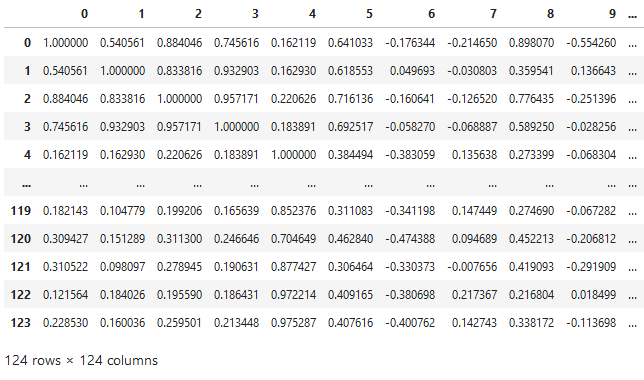
\includegraphics[width=\linewidth]{fig9.png}
  \caption{Correlation matrix for predictors in training set. Notice that there are many predictors with high correlation.}
  \label{fig:fig9}
\end{figure}

Thus a principal components analysis was performed to isolate a subset of variables which captured most of the variability within the data. Prior to this the data was also scaled so that each column had mean 0 and standard deviation 1. We found that the first 20 principal components captured about 99.999\% of variability in the training data. We elected to transform the training predictors dataframe so that the columns represented values of each principal component, and retain only these first 20 principal components to use as predictors.

\subsection{Model building and selection}

Having isolated the first 20 principal components to use as predictors, this was used along with the corresponding response variable (Density) to fit multiple machine learning models. Using the scikit-learn 0.22 Python library, we built 4 models in total: a Multiple Linear Regression model, a Boosting Regression model (AdaBoost), a Random Forest model, and a second Random Forest model where hyperparameter tuning was used. We then evaluated each model's performance using its R squared value when predicting on the test set which we set aside earlier. Identical transformations to that applied on the training set (using parameters of the training set) were applied to the testing set before evaluation. We then selected a final model using the testing set R squared values.

\section{Results}

A table comparing the performance of each model is presented in Figure \ref{fig:fig10}. Recall that the R squared is a value between 0 and 1 and captures the proportion of variability in the response that can be explained by the set of predictors, and is roughly indicative of how confident we can be in our predicted responses. As expected, the testing set accuracy (an estimate of out-of-sample accuracy) is lower than the training set accuracy since the model is prone to bias to the dataset it was trained on. Furthermore, we find that the testing set accuracy is \textit{significantly} lower than the training set accuracy in the Boosting and Random Forest models. This suggests high levels of bias and overfitting towards the training data, which can be attributed to the relatively small dataset size given that the Boosting and Random Forest algorithms require large amounts of data to be reliable. \\

We find that our Random Forest Regression models significantly outperform both the Multiple Linear Regression and Boosting Regression models. The use of hyperparameter tuning for the Random Forest model leads to only a slight increase in test set R squared but perfect fit on the training set (suggesting very strong levels of overfitting). We also want to avoid the use of slight improvements in the test set R squared to justify the model with hyperparameter tuning because we would then be introducing bias from information in the testing set. Thus, we select the first Random Forest Regression model as our final model with an estimated out-of-sample R squared of 0.36. A plot of the predicted responses from this model compared to the actual responses is given in Figure \ref{fig:fig11}.

\begin{figure}
\centering
  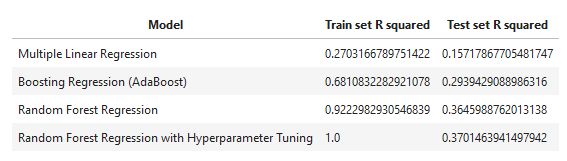
\includegraphics{fig10.png}
  \caption{A comparison of the performance of each machine learning model on the training and test sets using the R squared metric.}
  \label{fig:fig10}
\end{figure}

\begin{figure}
\centering
  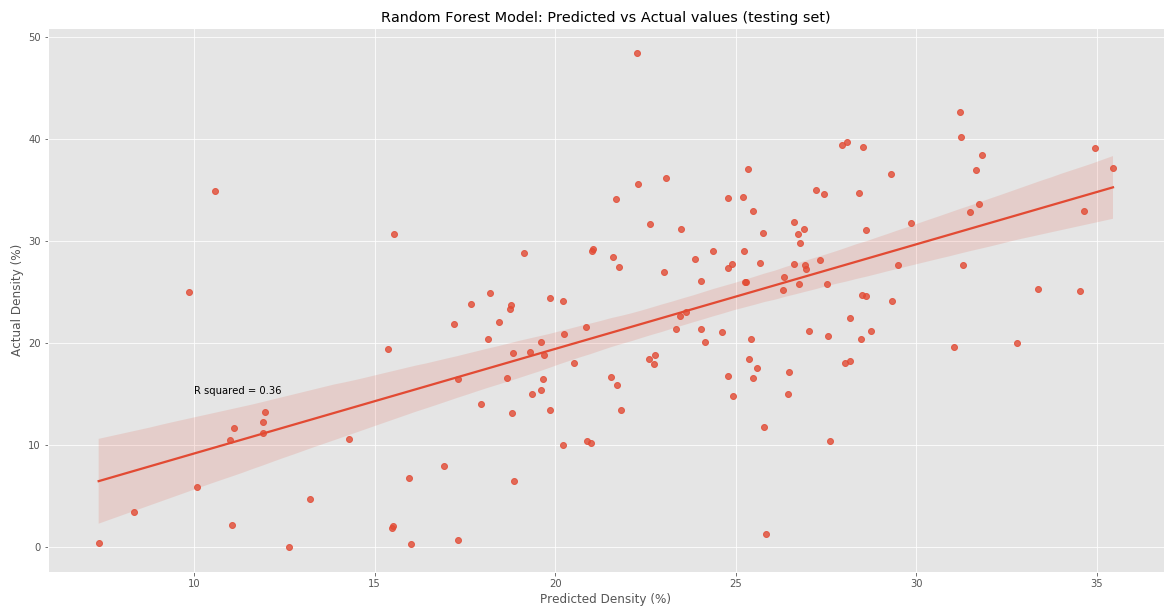
\includegraphics[width=\linewidth]{fig11.png}
  \caption{A regression plot comparing the predicted density of solar installation on the x-axis to the actual values on the y-axis.}
  \label{fig:fig11}
\end{figure}

\section{Discussion}

\subsection{Interpretation of analysis}

The analysis within this report was primarily to build a machine learning algorithm to predict solar installation rates (density) in each LGA based on demographic data and we have done this. The question of which demographic factors in particular are relevant in predicting solar installation rates is not answered, and as was mentioned is beyond the scope of this analysis. In this analysis we merely considered the question of using a large part of the combined information by demographic data to make predictions. In fact, the use of principal components analysis in our analysis obscures with our ability to answer questions pertaining to influential factors since it introduces interpretability issues. Where interpretability is concerned, an improvement that could be made is to use alternative dimension reduction techniques such as selecting the demographic variables with highest correlation with density or selecting those which have the lowest p-value when performing simple linear regression with density as the response. This would allow us to then evaluate the variable importance within our Random Forest model. \\

Insofar as this analysis is concerned, the results should be interpreted as:

\begin{itemize}
\item There is indeed a relationship between the solar installation rates and demographics of a LGA.
\item A machine learning algorithm can indeed be built to at least roughly predict the average solar installation rates of LGAs with similar demographics. The model that we built in particular captures around 36\% of the variability in solar installation rates via demographic information.
\end{itemize}

\subsection{Implications of results}

The developed model at current may be of only limited utility to policy makers or investors but could still potentially find use by researchers. The model does not have high enough predictive accuracy to reliably guide policy or investment decisions. Also, because the model was trained on demographic information from the 2016 census, its predictive ability is likely only limited to time periods around 2016. The model cannot account for social changes pertaining to solar installation, influential policy decisions, technological breakthroughs and other factors which may abruptly cause the model to be outdated. Instead, the density estimates can be used as \textit{indicators} regarding the relative likelihood to install solar within a LGA keeping all other things constant. Researchers could still potentially use this model as a tool to run simulations under different demographic scenarios to guide parts of their research (while it has yet to be outdated), or as a basis to build more highly predictive and time-robust machine learning models.

\subsection{Recommendations}

\begin{itemize}
\item Conduct qualitative research to elicit what are the most relevant demographic or even individual factors affecting solar installation.
\item Perform further data collection on a finer scale to create larger datasets for computational analysis, preferably after conducting the qualitative research so data of greater relevance is collected.
\end{itemize}

\section{Conclusion}

We were able to build a Random Forest Regression model that explains around 36\% of the variability in solar installation rates across different LGAs via demographical information. Through this model we demonstrated that there is indeed a relationship between solar installations rates and demographics. The built model is of insufficient accuracy for use in policy or investment but could be of use for researchers under marginal circumstances.

\medskip

\begin{thebibliography}{9}

\bibitem{ipcc} 
\url{https://www.ipcc.ch/report/renewable-energy-sources-and-climate-change-mitigation/}

\bibitem{pew} 
\url{https://www.pewresearch.org/fact-tank/2016/10/05/americans-strongly-favor-expanding-solar-power-to-help-address-costs-and-environmental-concerns/}

\bibitem{seia}
\url{https://www.seia.org/solar-industry-research-data}

\bibitem{geogov} 
\url{https://www.ga.gov.au/scientific-topics/energy/resources/other-renewable-energy-resources/solar-energy}

\bibitem{pvdata}
Australian PV Institute (APVI) Solar Map, funded by the Australian Renewable Energy Agency, accessed from pv-map.apvi.org.au on 19 February 2020. Dataset can be downloaded from \url{https://pv-map.apvi.org.au/historical#4/-26.67/134.12}.

\bibitem{apvi}
\url{http://apvi.org.au/about-us/}

\bibitem{ceg}
\url{http://www.cleanenergyregulator.gov.au/RET/Forms-and-resources/Postcode-data-for-small-scale-installations}

\bibitem{abspv}
\url{https://www.abs.gov.au/AUSSTATS/abs@.nsf/DetailsPage/1270.0.55.003July%202016?OpenDocument}

\bibitem{abs}
Australian Bureau of Statistics 2020, viewed 26 February 2020, \url{http://stat.data.abs.gov.au}.

\bibitem{tidy}
Wickham, H. (2014). Tidy Data. \textit{Journal of Statistical Software}, 59(10), 1-23.

\end{thebibliography}

\end{document}